\documentclass[../../diss.tex]{subfiles}
\begin{document}

\section{Technical core}%
\label{Section:WSTSSeparabilityCore}%

Both main results, \cref{Theorem:WSTSSeparability} and \cref{Theorem:DWSTSSeparability}, will follow from a technical core result.
We will prove this technical core in this section and then immediately obtain the regular separability of language-disjoint DWSTSes.
The result in the case of upward-compatible WSTSes will require more work.
To state the technical core, we need the notion of an inductive invariant that we will introduce in the following.

An \emph{invariant} is a property that holds for all reachable configurations.
We may see it the set of configurations that satisfy the property.
We will take this view in the rest of the section and see an invariant as a set of configurations containing the reachable ones.
In particular, the set of reachable configurations itself is an invariant.

We will be only interested in invariants that are \emph{safe}.
Normally, the notion of safety means that a certain set of \emph{bad} configurations cannot be reached.
Here, we will see the set of final configurations of an LTS as the set of configurations that should not be reachable:
A safe invariant is a set of configurations that contains all reachable configurations, but no final configuration.
Hence, a safe invariant is a certificate for language-emptiness.
If the language of an LTS is empty, then the set of reachable configurations itself is a safe invariant.

In the following, whenever we use the notion \emph{invariant}, we imply that it is safe.
The above discussion yields the following characterization:
For an LTS $\wsts = (\configs,T,\configs_\init,\configs_\final)$ with empty language, the invariants are precisely the sets $X$ so that
\[
    \reach{\wsts} \subseteq X \subseteq \configs \setminus \configs_\final
    \ .
\]
In particular, $\reach{\wsts}$ and the complement of $\configs_\final$ are invariants.

When checking whether a given set $X$ (representing some property) is an invariant, it is useful to impose a restriction that makes this task easier.
We call an invariant \emph{inductive} if for any configuration in the invariant, all its successors are also in the invariant: If $c \in X$, then $\post{}{\Sigma}{c} \subseteq X$.
This property simplifies the check because it can now be conducted in a local fashion: One checks that if a configuration satisfies the property defining the invariant, then the property still holds after doing a step in the transition system.
Invariants, and inductive invariants in particular, are a standard technique used for safety verification of programs~\cite{MannaP95}.

Checking whether a set $X$ is an inductive invariant amounts to checking (1)~that $X$ contains the initial configurations, (2)~that if $c \in X$, then $\post{}{\Sigma}{c} \subseteq X$, and that (3)~$X \cap \configs_\final = \emptyset$.
Properties~(1) and~(2) together imply that $X$ contains the reachable configurations.

While $\reach{\wsts}$ is always an inductive invariant if the given LTS has empty language, the same is not true for $\configs \setminus \configs_\final$.
It may contain the predecessor of a final configuration, which violates inductivity.
We exclude all ancestors of final configurations and obtain that $\configs \setminus \reachrev{W}$ is the greatest inductive invariant.
The inductive invariants of an LTS with empty language are exactly the inductive sets $X$ with
\[
    \reach{\wsts} \subseteq X \subseteq \configs \setminus \reachrev{W}
    \ .
\]

In the case of ordered LTS, we can additionally require $X$ to be downward closed.
In fact, if $X$ is an inductive invariant, then so is its downward closure $\dc{X}$.
Condition~(1) is maintained when adding configurations, Condition~(3) is maintained since we assume the set of final configurations to be upward closed.
For inductivity, assume that $c \in \dc{X}$, \ie $c \leq c'$ for some $c' \in X$.
Using upward compatibility, we have that for any $c \tow{a} d$, there is some $c' \tow{a} d'$ with $d \leq d'$.
We have $d' \in \post{}{\Sigma}{c'} \subseteq X \subseteq \dc{X}$ by assumption and conclude $d \in \dc{X}$ since $\dc{X}$ is downward closed.

The above discussion justifies the following definition of inductive invariants in the case of ordered LTS.\@

\begin{definition}
    An \emph{inductive invariant} for an ordered LTS $\wsts = (\configs,\leq,T,\configs_\init,\configs_\final)$ is a downward-closed set $X \subseteq \configs$ with
    (1)~$\configs_\init \subseteq X$,
    (2)~Safety:~$X \cap \configs_\final = \emptyset$, and
    (3)~Inductivity:~$\post{\wsts}{\Sigma}{X} \subseteq X$.
\end{definition}

An inductive invariant exists if and only if $\lang{\wsts}$ is empty.
If $\lang{\wsts}$ is empty, then the downward-closure of the reachable configurations $\dc{\reach{\wsts}}$ is the least, and the configurations that are not the predecessor of a final configuration $\configs \setminus \reachrev{W}$ is the greatest inductive invariant.
Note that the latter set is always downward closed by upward compatibility, while $\reach{\wsts}$ may not be downward closed if $\wsts$ is not internally downward closed.


In the following, we want to transform an inductive invariant for the product of two language-disjoint WSTSes into a regular separator for their languages.
This will only work if the inductive invariant has a certain finite representation.

\begin{definition}
    An inductive invariant $X$ is \emph{finitely represented} if $X = \dc{Q}$ for a finite set $Q$ of configurations.
\end{definition}

We have explained in \cref{Chapter:WSTSExpressiveness} that requiring a downward-closed set to be the downward closure of finitely many elements imposes a restriction.
Consider for example a Petri net with two places $p_1, p_2$.
The initial marking assigns no tokens, the final marking requires a token on the second place.
This means that the set of final configuration is $\N \times (\N \setminus \set{0})$.
There is a single transition that requires no tokens and produces a token on the first place.
Obviously, the set of configurations reachable in the associated WSTS is $\N \times \set{0}$.
To be precise, $\N \times \set{0}$ is a downward-closed safe inductive invariant, and it is the only safe invariant.
Any smaller set does not contain all reachable configurations, any bigger set contains a final configuration.
However, this invariant is not finitely represented as there is no finite set of numbers whose downward closure is $\N$.

Not every inductive invariant being finitely represented is a problem that we will need to overcome later.
For now, let us use the notion to state the core result.

\begin{theorem}%
\label{Theorem:WSTSSeparabilityCore}%
    Let $\wsts$ and $\wstsprime$ be language-disjoint ordered LTSes, one of them deterministic, such that their product $\wsts \times \wstsprime$ admits a finitely represented inductive invariant $\dc{Q}$.
    Then $\wsts$ and $\wstsprime$ are regularly separable by the language of a finite automaton with $Q$ as its set of states.
\end{theorem}

% The theorem is interesting in that it relates a property of the configurations of LTSes to a property of their languages.
One might wonder why the result talks about ordered LTSes instead of WSTSes.
The reason is that when we apply the result, we will first enforce the existence of a finitely represented invariant by applying a preprocessing step.
This step will turn the given (D)WSTSes into language-equivalent ordered LTSes that may not be (D)WSTSes in general.

We turn to the proof of \cref{Theorem:WSTSSeparabilityCore}.
Let $\wsts = (\configs,\leq,T,\configs_\init,\configs_\final)$ and $\wstsprime = (\configs',\leq',T',\configs_\init',\configs_\final')$ be the given WSTSes.
We assume that their languages are disjoint, $\lang{\wsts} \cap \lang{\wstsprime} = \emptyset$, and that $\wstsprime$ is deterministic.
We consider their product
\[
    \prodwsts = \wsts \times \wstsprime = (\prodconfigs,\prodT,\prodleq,\prodconfigs_\init,\prodconfigs_\final)
    \ ,
\]
and note that $\lang{\prodwsts} = \emptyset$ by assumption.
Let $Q \subseteq \prodconfigs$ be a finite set such that $\dc{Q}$ is an inductive invariant for $\prodwsts$.

We construct an automaton $A$ that has $Q$ as its set of states.
Its language will be a regular separator for the languages of the two given WSTSes.
To be precise, it will contain $\lang{\wsts}$ and be disjoint from $\lang{\wstsprime}$.
Before elaborating on its properties, we explain the construction.
\nb{Intuitively}, $A$ overapproximates the product WSTS $\prodwsts$ using the configurations from $Q$.
Note that the configurations of $\prodwsts$ (and hence the states of $A$) are tuples of configurations of the original WSTSes.


\begin{definition}%
\label{Definition:WSTSSeparabilityAutomaton}%
    The \emph{separating automaton induced by $Q$} is $A = (Q,\to,Q_\init,Q_\final)$.
    A state is initial if it is larger than some initial configuration of $\prodwsts$,
    \[
        Q_\init = \Set{ (q,q') \in Q }{ (c,c') \prodleq (q,q') \text{ for some } (c,c') \in \prodconfigs_\init}
        \ .
    \]
    A state is final if its $\wsts$-component is final,
    \[
        Q_\final = \Set{ (q,q') \in Q}{ q \in \configs_\final}
        \ .
    \]
    The transition relation of $A$ overapproximates the transition relation of $\prodwsts$ as follows:
    \[
        (q,q') \tow{a} (p,p') \text{ in } A
        \quad \textiff \quad
        (q,q') \tow{a} (c,c') \text{ in } \prodwsts \text{ for some } (c,c') \prodleq (p,p')
        \ .
    \]
\end{definition}

The latter part of the definition means that if $(q,q') \tow{a} (c,c')$ is a transition of the product and $(q,q') \in Q$, then $A$ can overapproximate this transition using any state $(p,p') \in Q$ with $(c,c') \prodleq (p,p')$.
This is depicted in \cref{Figure:SeparabilityAutomaton}.
We do not impose any precision requirement, but we could obviously require $Q$ to be an antichain.
The fact that $\dc{Q}$ is an inductive invariant will be sufficient to prove the correctness of the construction.

\begin{figure}[t]
   \centering%
   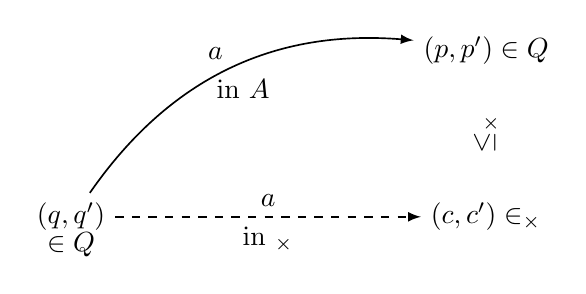
\begin{tikzpicture}[->,>=latex,semithick]

\node (Q) {$(q,q')$};
\node [below of=Q, node distance=1em] {$\in Q$};

\node (C) [right of=Q, node distance=15em] {$(c,c') \in \wsts_\times$};

\node (P) [above of=C, node distance=6em] {$(p,p') \in Q$};

\node [above of=C, node distance=3em, rotate=90] {$\leq_\times$};

\path [->,dashed]
    (Q) edge node [above] {$a$} node [below] {in $\wsts_\times$}
    (C)
;

\path [->]
    (Q) edge [bend left] node [above,xshift=-0.5em] {$a$} node [below,xshift=0.5em] {in $A$}
    (P)
;

\end{tikzpicture}
%
   \caption{The transition relation of the separating automaton $A$.}%
   \label{Figure:SeparabilityAutomaton}%
\end{figure}

\begin{remark*}
Note that we are dealing with an NFA with multiple initial states here.
We have already explained in \cref{Section:DescriptiveComplexity} that such an NFA can be transformed into an NFA with a unique initial state while introducing a single new state.
\end{remark*}

To prove that $A$ is indeed a separating automaton, we need to show $\lang{\wsts} \subseteq \lang{A}$ and $\lang{\wstsprime} \cap \lang{A} = \emptyset$.
We will prove the following:
\begin{itemize}
    \item Any computation of $\wsts$ can be embedded into a computation of $\prodwsts$, and this computation in turn is overapproximated by a run of $A$.
    \item Any run of $A$ on some word $w$, projected to the $\wstsprime$-component, overapproximates the unique computation of $\wstsprime$ for $w$.
\end{itemize}

From the first property, we get the inclusion $\lang{\wsts} \subseteq \lang{A}$.
Here, it is sufficient to assume that $\wstsprime$ is complete to obtain that any computation of $\wsts$ can be embedded into a computation of the product system.
From the second property, we get the disjointness $\lang{\wstsprime} \cap \lang{A} = \emptyset$.
For this statement to hold, it is important that $\wstsprime$ is deterministic.
Otherwise, the run of $A$ could overapproximate a non-accepting computation of $\wstsprime$ although an accepting one exists.

We proceed to formally state and prove the two properties, and conclude that $\lang{A}$ is a regular separator, which completes the proof of \cref{Theorem:WSTSSeparabilityCore}.
We start with a technical lemma that will be needed to establish $\lang{W} \subseteq \lang{A}$.

\begin{lemma}%
\label{Lemma:WSTSInclusion}%
    \begin{thmenumerate}[a)]
        \item~If $c \in \reach{\wsts}{w}$, then $(c,c') \in \reach{\prodwsts}{w}$ for some $c'$.
        \item~If $(c,c') \in \reach{\prodwsts}{w}$, then $(q,q') \in \reach{A}{w}$ for some $(q,q') \in Q$ with $(c,c') \prodleq (q,q')$.
    \end{thmenumerate}
\end{lemma}

\begin{proof}
    For Part~a), we have that $c'$ is in fact predetermined to be the unique configuration $\reach{\wstsprime}{w}$ since $\wstsprime$ is deterministic.
    Formally, we prove the statement by induction on $w$.
    In the base case, we have that $c \in \configs_\init = \reach{\wsts}{\eps}$ is an initial configuration of $\wsts$.
    We choose $c' = \reach{\wstsprime}{\eps}$ as the unique initial configuration of $\wstsprime$.
    By the definition of the synchronized product, we have $(c,c') \in \prodconfigs_\init = \reach{\prodwsts}{\eps}$ as desired.
    For the inductive step, consider $w.a$.
    A configuration $c \in \reach{\wsts}{w.a}$ is an $a$-successor of some configuration $d \in \reach{\wsts}{w}$.
    By induction, we have $(d,d') \in \reach{\prodwsts}{w}$.
    Since $\wstsprime$ is deterministic, there is a unique configuration $c' = \reach{\wstsprime}{w.a}$ that is the $a$-successor of $d'$.
    By the definition of the transition relation of the synchronized product, we have $(d,d') \tow{a} (c,c')$ in $\prodwsts$, and hence $(d,d') \in \reach{\prodwsts}{w.a}$ as desired.

    For Part~b), we use that an inductive invariant has to contain all reachable configurations of the system.
    Formally, we show the statement by induction on $w$.
    In the base case, we have that $(c,c') = \reach{\prodwsts}{\eps}$ is an initial configuration of the product system.
    By Property~(1) of being an invariant, this means $(c,c') \in \dc{Q}$.
    Hence, $Q$ contains some state $(q,q')$ with $(c,c') \prodleq (q,q')$.
    By the definition of the initial state of $A$, we have $(q,q') \in Q_\init = \reach{A}{\eps}$ as required.
    For the inductive step, consider $w.a$.
    Any configuration $(d,d') \in \reach{\prodwsts}{w.a}$ can be written as an $a$-successor of a configuration $(c,c') \in \reach{\prodwsts}{w}$, \ie $(c,c') \tow{a} (d,d')$ in $\prodwsts$.
    By induction, we obtain that there is some state $(q,q') \in \reach{A}{w}$ with $(c,c') \prodleq (q,q')$.
    Using upward compatibility, we get that there is some $(e,e')$ with $(q,q') \tow{a} (e,e')$ in $\prodwsts$ and $(d,d') \leq (e,e')$
    By inductivity, Property~(3) of being an inductive invariant, we have $\post{\prodwsts}{\Sigma}{\dc{Q}} \subseteq \dc{Q}$.
    Since $(q,q') \in Q \subseteq \dc{Q}$, we also obtain $(e,e') \in \dc{Q}$.
    Hence, there is some $(p,p') \in Q$ with $(d,d') \prodleq (e,e') \prodleq (p,p')$.
    By the definition of the transition relation of $A$, we have $(q,q') \tow{a} (p,p')$ in $A$ as this transition overapproximates the transition $(q,q') \tow{a} (e,e')$ of $\prodwsts$.
    We conclude $(p,p') \in \post{A}{a}{\reach{A}{w}} = \reach{A}{w.a}$ and $(d,d') \prodleq (p,p')$ as desired.
\end{proof}

With this lemma at hand, we can immediately conclude that the language of $A$ contains the language of $\wsts$.

\begin{proposition}%
\label{Proposition:WSTSInclusion}%
    $\lang{\wsts} \subseteq \lang{A}$.
\end{proposition}

\begin{proof}
    Assume that $w \in \lang{\wsts}$, \ie $c \tow{w} d$ for some $c \in \configs_\init$ and $d \in \configs_\final$.
    By using Statement~(1) of \cref{Lemma:WSTSInclusion}, we obtain that $(d,d') \in \reach{\prodwsts}{w}$ for some $d'$.
    Using Statement~(2) of the same lemma, we get that $(q,q') \in \reach{A}{w}$ for a tuple $(q,q') \in Q$ with $(d,d') \prodleq (q,q')$.
    Since $d \in \configs_\final$ and $\configs_\final$ is upward closed, we have $q' \in \configs_\final$ and hence $(q,q') \in Q_\final$.
    We conclude that $A$ has an accepting run on word $w$ as desired.
\end{proof}

We now show that every run of the automaton on some word overapproximates in its second component the unique run of $\wstsprime$ ob that word.

\begin{lemma}%
\label{Lemma:WSTSDisjointness}%
    For every $w \in \Sigma^*$ and every $(q, q') \in \reach{A}{w}$ we have $\reach{\wstsprime}{w} \leq' q'$.
\end{lemma}

\begin{proof}
    We proceed by induction on $w$.
    In the base case, we have that $(q,q') \in \reach{A}{\eps} = Q_\init$ is an initial state of $A$.
    By definition, this means $(c,c') \prodleq (q,q')$ for some initial configuration $(c,c')$ of $\prodwsts$.
    Again by definition we have that $c' \in \configs'_\init$ is the unique initial configuration of $\wstsprime$.
    Hence, we have $\reach{\wstsprime}{\eps} \leq' q'$.

    For the inductive step, consider $w.a$.
    We may write $(p,p') \in \reach{A}{w.a}$ as an $a$-successor of some state $(q,q') \in \reach{A}{w}$.
    This means that there is some transition $(q,q') \tow{a} (d,d')$ of the product system with $(d,d') \leq (p,p')$.
    Using induction, we get $\reach{\wstsprime}{w} \leq q'$.
    By the definition of the transition relation of the product system, we have that $d' = \reach{\wstsprime}{w.a}$ is the unique configuration reached by $\wstsprime$ when reading $w.a$, and we have $d' \leq p'$ as required.
\end{proof}

We use this lemma to conclude that the languages of $A$ and $\wsts'$ are disjoint.

\begin{proposition}%
\label{Proposition:WSTSDisjointness}%
    $\lang{A} \cap \lang{\wstsprime} = \emptyset$.
\end{proposition}

\begin{proof}
    Towards a contradiction, assume that $w \in \lang{A} \cap \lang{\wstsprime}$ is a counterexample to disjointness.
    Since $w \in \lang{A}$, there is some accepting state $(q,q') \in \reach{A}{w} \cap Q_\final$ of $A$ that can be reached by processing $w$.
    Note that $(q,q') \in Q_\final$ means that $q \in \configs_\final$ is a final configuration of the first WSTS by definition.
    Similarly, $w \in \lang{\wstsprime}$ means that the unique configuration $\reach{\wstsprime}{w}$ that $\wstsprime$ reaches after processing $w$ is final, \ie $\reach{\wstsprime}{w} \in \configs_\final'$.

    Using \cref{Lemma:WSTSDisjointness}, we obtain that $\reach{\wstsprime}{w} \leq' q'$.
    The set of final configuration of a WSTS is upward closed, so we can conclude $q' \in \configs_\final'$.
    Altogether, we obtain that $(q,q') \in \configs_\final \times \configs'_\final = \prodconfigs_\final$ is a final configuration of the product system.
    Furthermore, $(q,q')$ is an element of $Q$ since it is a state of $A$.
    This is a contradiction to the assumption that $\dc{Q}$ is an inductive invariant that satisfies safety, \ie $\dc{Q} \cap \ \prodconfigs_\final = \emptyset$.
\end{proof}

The Propositions~\ref{Proposition:WSTSDisjointness} and~\ref{Proposition:WSTSDisjointness} together show that the language of $A$ is a regular separator for the languages of $\wsts$ and $\wstsprime$.
Hence, the proof of \cref{Theorem:WSTSSeparabilityCore} is completed.


\paragraph{Applying the core result to obtain regular separability for DWSTSes}

We conclude this section by showing how we can use \cref{Theorem:WSTSSeparabilityCore} to show our main result in the case of DWSTSes.
Recall that \cref{Theorem:DWSTSSeparability} states that the languages of any two language-disjoint DWSTSes, one of them deterministic, are regularly separable.

Our core result speaks of upward-compatible LTSes.
To bridge the gap, we dualize the given DWSTSes by considering the opposite orders.
This process turns a downward-compatible DWSTS into an upward-compatible LTS that may not be well-quasi ordered, which is not a problem in this case.
Additionally, the dualization means that any downward-closed set in the product of the dualized DWSTSes is an upward closed set in the product of the original DWSTSes.
We can use that upward-closed sets in a WQO can always be written as the upward closure of finitely many elements, which makes the requirement of a finitely represented invariant trivial.

\begin{proof}[Proof of \cref{Theorem:DWSTSSeparability}]
    Let $\dwsts = (\configs,\leq,T,\configs_\init,\configs_\final)$ and $\dwsts' = (\configs',\leq',T',\configs_\init',\configs_\final')$ be the given language-disjoint DWSTSes where $\dwsts'$ is deterministic.
    We consider the opposite orders $\geq$ and $\geq'$, obtaining the (upward-compatible) ordered LTS $\dwsts^{-1} = (\configs,\geq,T,\configs_\init,\configs_\final)$ and $\dwsts^{\prime-1} = (\configs',\geq',T',\configs_\init',\configs_\final')$.
    Note that these indeed satisfy the requirements:
    For example, $\configs_\final$ being downward closed with respect to $\leq$ means that it is upward closed with respect to the opposite order.
    The downward-compatibility of $T$ (\wrt $\leq$) implies the upward-compatibility of $T$ \wrt $\geq$.
    Obviously, the languages and the fact that $\dwsts^{\prime-1}$ is deterministic remain unchanged.
    Hence, $\dwsts^{-1}$ and $\dwsts^{\prime-1}$ are language-disjoint ordered LTS and one of them is deterministic.

    To be able to apply \cref{Theorem:WSTSSeparabilityCore}, we need to find a finitely represented inductive invariant for $\dwsts_\times^{-1} = \dwsts^{-1} \times \dwsts^{\prime-1}$.
    We claim that the downward closure of the set of reachable configurations
    \[
        X = \dc{\reach{\dwsts_\times^{-1}}}
    \]
    is such a finitely represented invariant, where the downward closure is taken with respect to the product of the orders $\geq$ and $\geq'$.
    When we did introduce invariants, we have already discussed that for an ordered LTS with empty language, this set will always be an inductive invariant.
    To see that it is finitely represented, we first observe that $X$ is also the downward closure (with respect to the product of $\geq$ and $\geq'$) of the reachable configurations in the product of the original DWSTSes.
    In a second step, we note that the opposite order of the product of $\geq$ and $\geq'$ is actually the product of $\leq$ and $\leq'$.
    Hence, the downward closure with respect to the product of $\geq$ and $\geq'$ is the upward closure with respect to the product of the original orders.
    We may write
    $X = \ucwrt{\reach{\dwsts \times \dwsts'}}{\leq_\times}$.

    Since $\leq$ and $\leq'$ are WQOs, so is their product by \cref{Lemma:WSTSDickson}.
    By Property~(\ref{Property:WQOFiniteBasis}) of being a WQO, see \cref{Lemma:WQOProperties}, every upward-closed set can be written as the upward closure of finitely many elements.
    We obtain that $X = \ucwrt{\set{x_1, \ldots, x_k}}{\leq_\times}$ for suitable $x_1, \ldots, x_k \in \reach{\dwsts \times \dwsts'}$.
    In terms of the product of the opposite orders, we obtain that $X$ is the downward closure of $\set{x_1, \ldots, x_k}$, proving that $X$ is finitely represented.

    Hence, we have that $X$ is a finitely represented inductive invariant for $\dwsts_\times^{-1}$, so \cref{Theorem:WSTSSeparabilityCore} yields that $\lang{\dwsts^{-1}} = \lang{\dwsts}$ and $\lang{\dwsts^{\prime-1}} = \lang{\dwsts'}$ are regularly separable as desired.
\end{proof}

\end{document}
